\begin{auf}
    287
\end{auf}
In ein strömendes Gewässer wird senkrecht von oben ein Staurohr so hineingehalten, dass der unter Wasser befindliche, im rechten Winkel gekrümmte Schenkel gegen die Strömung gerichtet ist. Das Wasser im Rohr steht um $\Delta h=10.0cm$ über der freien Wasseroberfläche. Wie groß ist die Strömungsgeschwindigkeit $v$?
\begin{figure}[h]
    \centering
    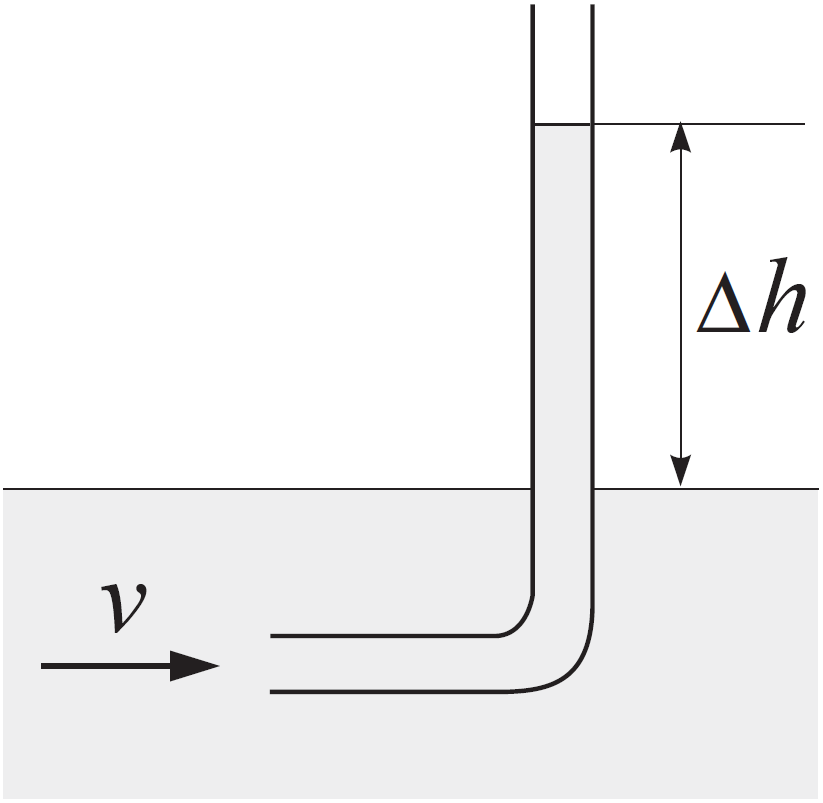
\includegraphics[height=5cm]{images/287_0.png}
    \caption{Versuchsaufbau Aufgabe 287}
\end{figure}